
\documentclass[a4paper, 12pt]{article}
\usepackage[a4paper,margin=0.9in]{geometry}
\usepackage[utf8]{inputenc}
\usepackage[frenchb]{babel}
\usepackage{indentfirst}
\usepackage{dirtree}
\usepackage{tikz}
\usepackage{amsmath}
\usepackage{framed}
\usepackage{parskip}
\usepackage{calc}
\usepackage{subfig}
\usepackage{hyperref}
\usepackage[toc,page]{appendix}
\usepackage{parskip}
\usepackage{listings}
\usepackage{color}
\usepackage{verbatim}
\usepackage{graphicx}
\usetikzlibrary{shapes,arrows}
\usetikzlibrary{trees}
\newcommand*{\xml}[1]{\texttt{<#1>}}

\setlength{\parskip}{12pt}

\title{Réseau Sémantique à partir d'un dictionnaire}
\author{Bawden Rachel, Brogniez Caroline et Parslow Nicholas}
\date{}

\begin{document}
\tikzstyle{every node}=[thick,anchor=west]
\tikzstyle{selected}=[draw=red,fill=red!30]

\tikzstyle{decision} = [diamond, draw, fill=blue!20, 
    text width=4.5em, text badly centered, node distance=3cm, inner sep=0pt]
\tikzstyle{block} = [rectangle, draw, fill=blue!20, 
    text width=5em, text centered, rounded corners, minimum height=4em]
\tikzstyle{line} = [draw, -latex']
\tikzstyle{cloud} = [draw, ellipse,fill=red!20, node distance=3cm,
    minimum height=2em]

\maketitle


\section{Objectifs}



\section{La Conception du Graphe}

L'idée de base pour un reseau semantique est de construire un graphe avec
les concepts pour noeuds et les liens entre les concepts comme arrêts.
Il exist deux approches générales à la construction. Premièrement, à
partir d'un dictionnaire, et deuxièment, à partir d'un corpus.
Un corpus a l'avantage de contenir les vraies utilisations des mots non-biasé
par les selections des auteurs, et aussi une grande
quantité d'utilisations, mais au même temps exige un algorithme non-supervisé pour la
désambiguisation et un autre algorithme pour la conversion de collocation en lien sémantique.
Word2Vec \hyperref[bib:word2vec]{[~\ref*{bib:word2vec}]} de
google réprésente le point actuel de cet approche.
Par contre, le dictionnaire, même si plus petit, donne plus
d'information sur les mots rares et possède déjà des liens sémantiques explicites entre
les mots.

L'utilisation d'un dictionnaire dans les tâches semantiques computationnelles
existe depuis les années 60 \hyperref[bib:olnyetal]{[~\ref*{bib:olnyetal}]}.
La construction d'un réseau sémantique à partir d'un dictionnaire (par exemple
en français \hyperref[bib:gaumeetal]{[~\ref*{bib:gaumeetal}]},
\hyperref[bib:mulleretal]{[~\ref*{bib:mulleretal}]}) est possible 
grâce à la structure des dictionnaires qui permet de faire ressortir des liens 
sémantiques. La structure en sens, sous-sens, définitions, et exemples, parmi 
d'autres informations, mais aussi la structure interne des définitions contient 
une régularité qu'il est important d'exploiter au maximum. Nous tenons donc à 
conserver le plus possible cette structure dans la transformation de dictionnaire 
en graphe. Un graphe est défini formellement comme un ensemble de sommets et un 
ensemble d'arcs qui relient une paire de sommets.

\[
G = <S, A>
\]

Pour représenter un dictionnaire par un graphe, nous considérons que les 
sommets peuvent être les mots individuels du dictionnaire ou même les niveaux 
intermédiaires de la structure tels que `exemple', `définition', `synonyme', 
`antonyme' etc. Les arcs sont alors les liens qui lient les différents éléments 
d'une entrée de dictionnaire et permettraient de trouver un lien entre un 
lexème donné et la manière dont il est décrit dans son entrée du dictionnaire.

Le graphe d'un reseau sémantique est connu d'exhiber les propriétés `Small World'
\hyperref[bib:veronis]{[~\ref*{bib:veronis}]} -
terme qui existe depuis l'experience fameux de Travers et Milgram
\hyperref[bib:traversmilgram]{[~\ref*{bib:traversmilgram}]}.
Watts et Strogatz \hyperref[bib:wattsstrogatz]{[~\ref*{bib:wattsstrogatz}]}
ont défini les propriétés d'un graphe `Small World' ainsi:
Si un graphe possède $N$ noeuds, et $d_{min}(i,j)$ est la distance minimum
entre noeuds $i$ et $j$, le `Characteristic Path Length' $L$ se défini par:
$$L = \frac{1}{N(N-1)} \sum\limits_{i\ne j} d_{min}(i,j) $$
et si pour un noeud $i$, l'ensemble de ses voisins immédiats est $\Gamma (i)$
et le nombre d'arrêts entre ses voisins immédiats est $E(\Gamma (i))$
alors le `Clustering Co-efficient' $C$ se défini par:
$$C = \frac{1}{N}\sum\limits_{i=1}^N \frac{E(\Gamma (i))}{\binom{|\Gamma (i)|}{2}} $$
Autrement dit, $L$ est la moyenne des distances minimales entre chaque couple
de noeuds dans le graphe, et $C$ est la moyenne du ratio des liens entre les voisins d'un
noeud et le nombre maximum de liens possible.

Un graphe `Small World' est défini par les propriétés suivants:
$$L \sim L_{rand} \sim \frac{log(N)}{log(k)} $$
et
$$C >> C_{rand} \sim \frac{2k}{N} $$
où $k$ est le dégée moyenne des noeuds du graphe et $L_{rand}$ et $C_{rand}$ sont respectivement
le Characteristic Path Length et Clustering Co-efficient pour un graphe aléatoire.

Par conséquent, un graphe `Small World' n'est pas dense, mais a des distances entre les noeuds
très petites. Une autre conséquence démontré par Barabási et Albert
\hyperref[bib:barabasi]{[~\ref*{bib:barabasi}]} est que la distribution des dégrés
des noeuds suivre une loi de puissance:
$$ p(k) \propto k^{-\alpha}$$
où $p(k)$ est la probabilité d'un noeud quelconque d'avoir un dégré k, et
$\alpha$ s'approche à l'unité (\hyperref[bib:veronis]{[~\ref*{bib:veronis}]})

% make histograms here

\subsection{Remarques sur la terminologie}
Nous appelons `mot' toute unité minimale du lexique. Un mot peut être
soitfléchi, soit non-fléchi et par défaut nous faisons référence aux mots 
non-fléchis sous leur forme de dictionnaire. Par principe, nous restreignons le 
réseau aux lemmes, mais il est possible qu'il y apparaît des formes fléchies en 
cas de non-identification du lemme.

Par `entrée' de dictionnaire nous faisons référence à un groupe d'informations 
(catégories syntaxiques, sens, définitions, exemples etc.) associées à un mot 
donné. Par conséquent, le terme `entrée' peut aussi être utilisé pour dénoter 
le mot lui-même, et par extension les informations contenues pour ce mot donné.

La relation sémantique de synonymie est définie entre deux termes de la même 
catégorie de discours qui ont le même sens et qui peuvent donc être substitués 
l'un pour l'autre sans modifier le sens de la phrase. Cette définition pose 
évidemment des problèmes, surtout à cause du fait qu'il est toujours possible 
de trouver une différence de sens ou d'usage entre deux mots malgré le fait 
qu'ils soient habituellement classés en synonymes. Il est parfois souhaitable 
de parler de proche-synonymes au lieu de synonymes tout court. Néanmois, 
nous préférons utiliser le terme `synonyme' pour parler de ces cas, sans 
postuler de théorie sur les frontières de la synonymie. Par la suite, la 
synonymie sera définie en termes de relations attestées dans des ressources 
externes et nous nous reportons à ces références pour établir si deux mots sont 
en relation de synonymie ou pas.

De même pour les relations d'antonymie, d'hyperonymie et d'hyponymie. 
L'antonymie est définie comme la relation entre deux mots à sens opposé. 
L'hyperonymie entre un mot dont l'extension contient l'extension d'un autre mot 
(par exemple, `véhicule' est l'hypernym de `voiture'). L'hyponymie est la 
relation inverse d'hyperonymie, entre un mot dont l'extension est incluse dans 
l'extension d'un autre (pour reprendre le même exemple, `voiture' est un 
hyponyme de `véhicule').

[AUTRES DEFINITIIONS...]


\section{La structure des dictionnaires utilisés}

Les deux ressources qui seront utilisées sont le Wiktionnaire français en 
format XML du CLLE-ERSS dans le cadre du projet WiktionaryX 
\hyperref[bib:wikixml]{[~\ref*{bib:wikixml}]} et le Littré , qui est aussi 
disponible en format XML \hyperref[bib:littrexml]{[~\ref*{bib:littrexml}]}.

Les informations contenues dans les deux dictionnaires sont similaires. Chaque 
dictionnaire est organisé en entrées, et chaque entrée contient plusieurs 
définitions, des exemples, des synonymes et des informations grammaticales. Le 
wiktionnaire contient en plus d'autres relations sémantiques telles que 
l'antonymie, l'hyperonymie et l’hyponymie.

\subsection{Statistiques}

NOMBRE d'ENTREES
NOMBRE DE CATS SYNT DIFF
NOMBRE DE MOT-FORMES DIFF


\section{Pré-traitement}

Dans le but de pouvoir procéder à un traitement homogène des deux dictionnaires, 
une normalisation des deux formats était nécessaire. Ce pré-traitement a permis 
à la fois de supprimer certaines informations qui n'étaient pas utilisée par la 
suite et de convertir les balises et leur contenu en un format plus convenable 
pour notre traitement. Nous réunissons les deux structures dans un seul type de 
fichier XML avec les balises suivantes:

    \begin{itemize}
        \item[$\circ$] entry : un mot du dictionnaire (lexème)
        \item[$\circ$] pos : la catégorie syntaxique (il peut y en avoir 
plusieurs par lexème)
        \item[$\circ$] sense : le niveau hiérarchique représentant plusieurs 
        sens d'un même mot
        \item[$\circ$] subsense : le niveau hiérarchique représentant plusieurs 
        sous-sens d'un même sens global
        \item[$\circ$] def-text : le texte d'une défintion
        \item[$\circ$] semantic : l'emploi sémantique d'un mot (figuratif, 
        absolu etc.)
        \item[$\circ$] register : le registre du mot (familier, vulgaire, 
        soutenu etc.)
        \item[$\circ$] domain : le domaine sémantique du mot (géographie, 
        biologie, culinaire etc.)
        \item[$\circ$] refs : des références vers d'autres entrées lexicales
        \item[$\circ$] examples : des phrases exemples contenant le mot de 
        l'entrée lexicale
        \item[$\circ$] synonyms : synonymes de du mot de l'entrée
        \item[$\circ$] antonyms : antonymes de du mot de l'entrée
        \item[$\circ$] hyperonyms : hyperymes de du mot de l'entrée
        \item[$\circ$] hyponyms : hyponymes de du mot de l'entrée
    \end{itemize}
\bigskip

La DTD des fichiers XML normalisés se trouve dans l'appendice 
\hyperref[App:dtddico]{~\ref*{App:dtddico}}, 
avec les scripts de normalisation 
\hyperref[App:normlittre]{~\ref*{App:normlittre}} et 
\hyperref[App:normwiki]{~\ref*{App:normwiki}}. 
\hyperref[fig:XMLhierarchy]{Figure~\ref*{fig:XMLhierarchy}} illustre 
l'hiérarchie des balises, qui correspond aussi à la structure théorique du 
réseau.

\begin{figure}[!ht]
\centering
\def\svgwidth{\columnwidth}
\input{schema.pdf_tex}
\caption{L'hiérarchie des entrées définie pour les dictionnaires en XML}
\label{fig:XMLhierarchy}
\end{figure}


De légères différences existent entre les structures des deux dictionnaires. 
Tandis que la plupart des informations du Wiktionnaire sont localisées au niveau 
du 'sense', la plupart des informations du Littré sont localisées au niveau du 
'subsense', ce qui ne pose aucun problème pour la construction des deux réseaux.
\newline
\newline
En plus de la restructuration des fichiers XML, les dictionnaires ont été 
nettoyés pour convenir à nos besoins. Certaines balises contiennent trop 
d'informations ou des informations non-pertinentes. Par exemple, les balises des 
commentaires pour le Littré ne contiennent pas de contenu exploitable et les 
citations des textes anciens des mots vieillis qui risquent d'ajouter du bruit 
dans le réseau résultant. Les entrées sont ainsi réduites au schéma ci-dessus 
(\hyperref[fig:XMLhierarchy]{Figure~\ref*{fig:XMLhierarchy}}). Le Littré en 
particulier nécessite une étape importante de nettoyage, puisque des erreurs 
existent dans le balisage des données et un manque d'homogénéité dans la 
structuration des entrées risque de perturber la manière dont laquelle les 
relations sont établies entre les éléments qu'elles contiennent. Les catégories 
syntaxiques utilisées ne sont pas d'une liste énumérable et contiennent des 
descriptions plutôt littéraires. Cette étape de normalisation consistait aussi à 
traduire ces catégories syntaxiques en une liste plus formelle et identifiable.

Les définitions, exemples et autres informations dans les entrées étaient 
ensuite taggés et lemmatisés en utilisant l'outil MElt 
(\hyperref[bib:melt]{[~\ref*{bib:melt}]}). Cette étape est importante pour 
pouvoir relier les mots fléchis des définitions avec leurs lemmes tels qu'ils 
apparaissent dans les entrées et pour savoir de quelle catégorie syntaxique il 
s'agit. Le script XXX qui sert à tagger et lemmatiser les documents se trouvent 
dans l'annexe \hyperref[App:tag]{[~\ref*{App:tag}]}.

\begin{center}
\begin{tabular}{|l|c|c|c|}
\hline
              & totale & bien-taggés & assez-bien-taggés  \\
\hline
tout les mots & 155    & 131 (85\%)  & 139 (89\%)         \\
\hline
mots lexicaux & 87     & 75  (86\%)  & 78  (90\%)         \\
\hline
\end{tabular}
\end{center}

Table (XXXXX) montre que MELT est suffisament accuré d'environ 90\%
du temps. Un tag est `assez-bien-taggé' si notre conversion de tags
élimine la faute. Les mots lexicaux comprennent les verbes, noms,
adjectifs et adverbes, y compris ``être'' et ``avoir''
dans tous leurs formes, mais pas les prepositions.

MELT a des difficultés avec les définitions qui ont un structure
particulier au dictionnaire et donc ne sont pas des phrases complêts
par exemple:

$$Synonyme/ADJ/synonyme \;\; d'/P/de allegro/NC/allegro \;\; ./PONCT/.$$
$$<domain>marine/ADJ/marin$$
où nous voyons
\emph{form\_original / catégorie assigné par MELT / lemma assigné par MELT}
pour
chaque token dans la phrase. Les premiers mots de la phrase sont les
plus souvent affectés. MELT offre la possibilité de s'entrainer sur
un corpus particulier, alors une amélioration possible serait d'annoter
une partie de la dictionnaire manuellement et utiliser cette partie
pour l'entrainement. Il n'est pas clair par contre si le temps pour
faire une quantité suffissament grand vaudrait le gain.


\section{La représentation en graphe}


\subsection{La première version du graphe}

Les fichiers XML sont facilement transférables en représentation en graphe, 
puisqu'ils continennent une hiérarchie arborescente d'entrées.
En principe chaque niveau de la hiérarchie est représenté par un nœud différent 
avec des arcs qui lient chaque nœud à ses fils dans la hiérarchie, comme dans 
\hyperref[fig:XMLhierarchy]{Figure~\ref*{fig:XMLhierarchy}}. Cette 
représentation a l'avantage de préserver la structure hiérarchique d'origine.

En plus des arêtes descendantes qui existent dans le schéma 
\hyperref[fig:XMLhierarchy]{Figure~\ref*{fig:XMLhierarchy}}, nous établissons 
des arêtes montantes, afin de retrouver facilement la relation entre un mot qui 
apparaît dans une entrée et le lexème de l'entrée. Les poids sur ces arêtes ne 
sont pas les mêmes que les arêtes descendantes afin de retrouver une différence 
dans ces relations (Voir la pondération des relations pour plus de détails).


\subsubsection{Simplification de la structure}
En pratique, il est possible de surpasser d'un grand nombre de nœuds 
intermédiaires dans la hiérarchie en attribuant une arête directe entre une 
paire de mots dont le poids serait l'addition de toutes les valeurs des liens 
qui constituent le chemin entre les deux mots. Le choix des sommets est un 
compromis entre mettre le plus d'informations possibles dans le graphe et 
veiller à la non-explosion de la taille du graphe. Ceci n'est possible que 
parce que dans les tâches effectuées (détaillés dans la partie XXX), nous 
n'aurons jamais besoin d'extraire ces nœuds intermédiaires, même si nous 
souhaitons tenir compte de leur présence.

Ainsi, l'entrée dans \hyperref[fig:banane_full]{Figure~\ref*{fig:banane_full}} 
est simplifiée en l'entrée dans 
\hyperref[fig:banane_simple]{Figure~\ref*{fig:banane_simple}}:

\begin{figure}
\centering
\parbox{5cm}{
\def\svgscale{0.5}
\input{entry_banane_full.pdf_tex}
\caption{}
\label{fig:banane_full}}
\qquad
\begin{minipage}{5cm}
\def\svgscale{0.5}
\input{entry_banane_simple.pdf_tex}
\caption{}
\label{fig:banane_simple}
\end{minipage}
\end{figure}

Notons que nous préservons deux niveaux de hiérarchie pour le mot d'entrée : un 
contenant le mot seul et l'autre contenant aussi sa catégorie syntaxique. Ceci 
est un moyen d'assurer que le mot soit trouvable dans le réseau sans devoir 
spécifier une catégorie syntaxique particulière, tout en permettant de faire la 
distinction entre plusieurs catégories syntaxiques pour un mot donné. Chaque mot 
taggé à l'intérieur d'une entrée est ainsi lié à une version non-taggée qui 
représente le niveau 'entry' de ce mot, même s'il n'existe pas comme entrée dans 
le dictionnaire de départ.

Le résultat est donc un graphe qui contient deux sortes de nœuds: des mots 
non-taggés (correspondants au niveau entry') et des mots taggés (correspondant 
au niveau 'pos'), avec des relations pondérées selon le lien établi entre les 
deux mots dans le dictionnaire.

[IMAGE plein d'arêtes].

\subsection{Graphe minimaliste}

Pour trouver les distances à partir des mots non-taggés ou des ensembles
conceptuels, le premier graphe fonctionne bien. Par contre, pour
la désambiguisation, les noeuds de entry et pos ne sont pas convenables.
Tout d'abord, il faut au minimum, ajouter des noeuds correspondants aux sens
différents. Si on ignore la différence entre sens et sous-sens (En principe
cela devrait correspondre à celle de homonymie par rapport à polysemie,
mais malheureusement ce n'est pas une distinction constemment appliquée
dans les dictionnaires et alors difficile à incorporer), cela mène à un
graphe à trois niveaux : entrée, pos et définition.

Si on retient entrée le graphe va contenir une ambiguité inherente
entre les différents pos. Ce niveau n'aide pas à séparer les
sens parce que des liens vers les définitions doivent soit passer par
là (et alors avoir une ambiguité de plus), soit aller directement aux noeuds
pos et alors le niveau en haut est superflou. Vu que l'information
catégorielle est disponible avec une bonne précision avec MELT, nous nous
débarassons du niveau `entrée' et retient que les mot\_pos et les définitions.
Une autre manière d'y voir est de considerer que nous enlevons le lien direct
entre la phonétique et la sémantique. Par exemple, dans un tel graphe,
 le lien entre ``bleu''
en tant que adjectif et ``bleu'' en tant que nom n'est pas automatique.
Pour la majorité de mots ce ne pose pas de problème parce que si les deux
formes sont liés semantiquement l'un va apparaitre dans la définition
de l'autre et vice-versa, en plus si on regarde un mot en forme flechi,
normalement, il
faut l'avoir déjà désambiguisé categoriellement pour avoir trouver la forme
dictionnaire (l'entrée) donc en pratique ce n'est pas un niveau utile.

le graphe qui resulte ignore la phonétique, mais retient la syntaxe et
l'ambiguité forte sémantiquement. L'ambiguité est forte parce que chaque
définiton dans le dictionnaire contient des mots qui sont eux-mêmes
ambigüs. Ce graphe est parfaitment bipartie.
et pour éviter la cross-contamination des liens sémantiques des
définitions, il est orienté. 

La forme du graphe ressemble au graphe d'internet.

\begin{figure}
\centering
\parbox{5cm}{
\def\svgscale{0.5}
\input{Images/graph_shocker.pdf_tex}
\caption{}
\label{fig:graph_shocker}}
\end{figure}

Ce graphe contient un component très large et fortement connexe (SCC) (jaune),
une petite partie sortante (verte) qui contient des mots qui sont
utilisés dans les définitions mais qui ne possède pas une définition
eux-mêmes. La plupart d'eux sont des mots mal-taggés ou que MELT n'a
pas reconnu. La troisième partie (rouge) est la partie des mots qui
ont définitions mais qui ne sont jamais utilisés dans une définition
eux-même. Ils peuvent aussi avoir des mots non-définis dans leurs
définitions d'où les tendrils.

La partie sortant peut être reduit en regardant si le mot\_pos existe
dans le dictionnaire mais avec une autre catégorie. Ce procesus remplace
entre la moitié et un tiers de tels noeuds. (voir code merge\_rows XXXXX)
Il faut noter aussi, que la partie entrant est exactement comme une
phrase à l'extérieur du dictionnaire, c'est à dire que pour désambiguiser
le dictionnaire, on peut seulement se concentrer sur le componant
fortement connexe. Ce fait nous aide beaucoup parce que la taille du
graphe est si large.

\begin{tabular}{|l|c|c|c|}
\hline
             & Composant Sortant & SCC   & Composant Entrant \\
\hline
Graphe A     &  5195             & 64180 &  77742            \\
\hline
Graphe B     &  6248             & 63356 &  81181             \\
\hline
\end{tabular}


la table montre les tailles des composants pour un graphe sans ambiguité
(Graphe A), c'est le graphe avec seulement les prémieres définitions
choisies, et pour un graphe maximalement ambigue (Graphe B), c'est le graphe
où s'il y a un lien de noeud $i$ vers noeud $j$ et $j$ est une des
definitions possibles pour un mot $m$ alors le graphe contient aussi des
liens de $i$ vers toute autre définiton de $m$

\begin{tabular}{|l|c|c|c|c|c|c|c|}
\hline
Taille de sccs               & 1      & 2    & 3   & 4  & 5  & 6  & 7 \\
\hline
Graphe A Composant Sortant   & 5195   & -    & -   & -  & -  & -  & -  \\
Graphe A Composant Entrant   & 76484  & 990  & 184 & 62 & 18 & 1  & 3 \\
\hline
Graphe B Composant Sortant   & 6248   & -    & -   & -  & -  & -  & -  \\
Graphe B Composant Entrant   & 79881  & 1009 & 200 & 64 & 22 & 2  & 3  \\
\hline
\end{tabular}

Pour utiliser ce graphe pour resoudre l'ambigüité sémantique, il
faut tout d'abbord resoudre l'ambigüité interne propre à la graphe.
Parce que le graphe est bipartite, on peut enlever un niveau et remplacer
les arrets sans perdre les distances entre le niveau restant.

Premierement nous avons essayé de prendre seulement le sens de la
première définition (le poid des liens vers des autres définitions
alors étant zéro pour chaque utilisation). L'idée derriere est que
 les définitions sont écrites en
ordre d'importance et ca va alors souvent être la bonne choix. Un regarde
 sur le dictionnaire a démontré que ce n'est pas en fait le cas et une
solution si facile ne nous aide pas.

En principe la partie fortement connexe de la matrice peut
 se désambiguiser lui-même en regardant le flou de probabilité de
chaque noeud définition vers son noeud pos mère dans le graphe où tout les
probabilités entre un pos et ses définitions sont egaux, la définition la
plus prôche va avoir la plus grande probabilité de rentrer à sa mère dans
le graphe (figure XXXXXX).


\begin{figure}
\centering
\parbox{5cm}{
\def\svgscale{0.5}
\input{Images/graphloop.pdf_tex}
\caption{Un noeud pos $A$ a deux définitions: $B$ et $C$. La probabilité
la plus grande entre $p(B\rightarrow A)$ et $p(C\rightarrow A)$ détermine
le sens préféré.}
\label{fig:graphloop}}
\end{figure}

Il est même possible d'envisager un processus itérative par Expectation
Maximisation (EM) où la probabilité d'une transition se rédefinit à
chaque tour par (par exemple pour le graph dans figure XXXXX)
$$p_t(i\rightarrow j) = \frac{p(j\rightarrow i)}{\sum\limits_{k}p(k\rightarrow i)}$$
où la somme k est une élement des noeuds définitions pour le même pos que $j$.
Malheureusement le temps neccessaire pour cet algorithme était trop grand pour l'essayer avec nos ordinateurs actuels.


\section{La pondération des relations}

Pour injecter plus de sophistication dans le réseau, la distance entre deux mots 
ne se limite pas au nombre d'arêtes dans le chemin. Les arêtes sont pondérées 
selon le type de nœud sortant et entrant afin de distinguer les relations 
différentes qui peuvent exister à différents endroits de l'entrée. Contrairement 
aux réseaux sémantiques plus sophistiqués tels que WordNet 
\hyperref[bib:wordnet]{[~\ref*{bib:wordnet}]}, qui encodent des relations typées 
spécifiques, notre réseau se base sur un principe plus simple de pondération, 
avec des valeurs réelles assignées par rapport à l'emplacement des mots dans 
l'entrée du dictionnaire.

Les poids des arêtes font partie des paramètres du réseau et sont conservés 
dans un fichier de configuration externe (weight.config), les valeurs étant 
choisies pour optimiser le réseau pour une tâche particulière. L'optimisation 
sera discutée dans la partie [XXX]. Il existe un total de 42 liens différent 
avec un poids différent entre 0 et 1, un lien de 0 étant un 
lien non-existant dans le graphe.

Ci-dessus un exemple d'un extrait de ce fichier, qui se trouve dans l'annexe :

\begin{framed}
entry2pos = 0.01\newline
pos2entry = 0.01\newline
pos2sense = 0.01\newline
sense2pos = 0.01\newline
pos2syn = 0.01\newline
syn2pos = 0.01\newline
...\newline
sense2subsense = 0.001\newline
subsense2sense = 0.001\newline
subsense2deftext = 0.00001\newline
deftext2subsense = 0.00001\newline
subsense2semantic = 0\newline
\end{framed}

En plus de ces paramètres basés uniquement sur la structure des entrées, 
d'autres paramètres sont utilisés pour faire ressortir des informations 
lexicales en plus de ces relations déjà trouvées. Ces paramètres se trouvent 
dans un deuxième fichier de configuration, qui peut être modifié de la même 
façon que le fichier de poids. La différence est que l'utilisateur peut 
spécifier le type d'opération mathématique (ex: multiplication, addition etc.) à effectuer sur le poids d'origine. Chaque paramètre est écrit sur une seule ligne avec l'étape de la création du graphe à 
laquelle le paramètre sera implémenté, ainsi que d'autres options utilisées pour 
spécifier comment le paramètre peut être utilisé.

Etant donné un mot x et un mot y, où x est le mot d'entrée et y le mot de sa 
définition: le poids original entre x et y serait le poids spécifié entre un mot d'entrée et 
sa définition (c'est-à-dire entry2pos + pos2sense + sense2subsense + 
subsense2deftext). Ensuite ce poids peut être transformé de plusieurs façons:

\subsection{En fonction des propriétés catégorielles}
Pendant l'étape de préparation du graphe, avant la création de la matrice, les 
poids sont modifiés en fonction des propriétés catégorielles pour donner plus 
ou moins de poids à certaines catégories. Les paramètres sont de la forme 
suivante :
    \begin{framed}
        POS\_de\_y, POS\_de\_x, fichiers\_contextes, opération\_math, valeur
    \end{framed}

\subsubsection{Modification uniquement en fonction de la catégorie 
syntaxique du mot y.}
Ces paramètres servent à privilégier certaines catégories de mot par rapport à 
d'autres, en supposant que certaines catégories sont plus utiles pour établir 
des relations sémantiques. Ceci se fait en fonction des relations que nous souhaitons faire ressortir. Par exemple, il peut être plus pertinent de prendre en compte les adjectifs si ce sont des descriptions qui doivent ressortir et de donner plus d'importance aux verbes si ce sont des actions qu'il faut caractériser (une plus grande importance se traduisant par un plus petit poids). Un paramètre est spécifié pour 
chaque catégorie syntaxique afin d'établir des modifications relatives entre 
catégories. Par exemple, pour la catégorie \lq{adjectif}\rq: \lq{prepare: Adj, 
None, None, +, 0.6}\rq{} signifie que 0.6 est ajouté à tout noeud qui va vers un 
mot de catégorie \lq{Adj}\rq{}.

\subsubsection{Modification en fonction de la catégorie syntaxique du mot x, du 
mot y et d'un fichier de contextes spécifiques.} 
Jusqu'à présent le poids des relations a été fondé uniquement sur l'emplacement 
des mots y dans l'entrée et de leurs catégories syntaxiques. Mais il est aussi 
important d'analyser la structure des informations à l'intérieur des 
définitions, puisque les définitions font preuve d'une régularité qui permet de 
donner plus de poids à certains mots. Sans faire une analyse syntaxique complète 
des définitions, nous visons à cibler certains mots qui apparaissent dans un 
certain contexte afin de renforcer la relation entre le mot de l'entrée et ces 
mots cibles. La forme du paramètre dans le fichier de configuration est la même 
que pour les paramètres précédents, sauf que la deuxième option 
lq{POS\_de\_x}\rq{} est spécifiée, ainsi que le chemin vers le fichier de 
contextes légitimisants. Vu que les contextes sont des expressions qui aident
seulement à la définition, les mots lexiques qui font partie d'un contexte
retrouvé sont ignoré dans la construction du graphe. 

Nous jugeons nécessaire de spécifier la catégorie syntaxique du mot x ainsi que 
la catégorie du mot y. Ceci parce que la forme de la définition dépend en grande 
partie de la catégorie syntaxique du mot de l'entrée. La relation entre un 
mot x de catégorie \lq{nom}\rq{} et un mot y de catégorie \lq{nom}\rq{} n'est pas la même 
relation que celle entre un mot x de catégorie \lq{nom}\rq{} et un mot y de 
catégorie \lq{verbe}\rq.

Par exemple, pour un mot x de catégorie \lq{adverbe}\rq, il pourrait être 
pertinent de renforcer le lien entre x et y, si y est un adjectif qui apparaît 
dans le contexte \lq{d'une manière mot\_y}\rq.

\underline{Syntaxe}\newline
Nous définissons une syntaxe particulière pour représenter les contextes 
légitimisants. En général ce sont des séquences de mots précédant et/ou suivant 
le mot y en question, qui signale que ce mot doit être mis en valeur.\newline

\begin{itemize}
    \item{Les contextes précédents et suivants sont des séquences de mots. Ces 
    séquences peuvent contenir soit des mots-formes, soit des lemmes, ce qui 
    permet plus de flexibilité dans la rédaction des règles et de ne pas devoir 
    expliciter toutes les combinaisons de formes fléchies possibles.}

    \item{\# représente la position du mot y, ce qui permet de spécifier le 
    contexte précédent et le contexte suivant du mot.}

    \item{Les symboles \string^ et \$ représentent respectivement le début et 
    la fin de la phrase}

    \item{Un chiffre indique le nombre maximum de mots qui peuvent apparaître à 
    une position donnée, sans devoir spécifier la forme ou le lemme de ces mots. 
    Notez que ces mots ne peuvent pas être un signe de ponctuation ou de la 
    même catégorie syntaxique que le mot y. Ceci fait en sorte que ce soit 
    le premier mot de la catégorie recherchée qui est renforcée par ce 
    contexte.}

\end{itemize}

Par exemple, dans l'entrée du mot \lq{langoureusement}\rq{}, la définition 
\lq{d'une manière langoureuse}\rq{} et le contexte légitimisant \lq{de une manière 
\#}\rq{} permettrait de renforcer la relation entre \lq{} langoureusement\rq{} et \lq 
langoureux\rq{}, ce dernier apparaissant dans la position spécifiée par \#. Dans 
cet exemple, il n'y a pas de contexte suivant spécifié (puisqu'aucun mot ne suit 
le \#) et ceci est le cas dans la plupart des contextes, où le contexte 
précédent est le plus important. Pour simplifier les contextes, nous permettons 
de ne pas exprimer le \# et dans ce cas, la séquence de mots est considérée 
comme la séquence précédente du mot y. Pour reprendre l'exemple précédent, le 
contexte \lq{de une manière \#}\rq{} peut également être exprimé \lq{de une 
manière}\rq. Notons que si un contexte suivant est explicité, le \# est 
nécessaire.

Ci-dessous quelques exemples de contextes pour une paire de catégories pour les 
mots x et y:

\begin{table}[ht]
\centering
\begin{tabular}{|p{1cm}|p{1cm}|p{5.5cm}|p{8cm}|}
\hline
POS de x & POS de y & Contexte & Description\\[0.5ex]
\hline
Adj & Adj & . \# . & Un adjectif entre deux points \\
Nom & Nom & \string^ \# ,  & Un nom au début de la définition, suivi d'une 
virgule \\
Nom & Nom & synonyme de & Un nom qui suit la séquence \lq{synonyme de}\rq \\
Adj & Verbe & en parlant de une personne qui 3 & Un verbe qui suit la séquence 
\lq{en parlant de une personne qui}\rq avec un maximum de 3 mots intervenants 
qui ne sont pas de catégorie PONCT ou V \\
Adj & Nom & qui a des rapports avec 2 & Un nom qui suit la séquence \lq{qui a 
des rapports avec}\rq avec un maximum de 2 mots intervenants qui ne sont pas de 
catégorie PONCT ou N \\ [1ex]
\hline
\end{tabular}
\caption{Quelques exemples de contextes légitimisants}
\label{table:nonlin}
\end{table}


Les contextes ont été choisis en analysant les entrées de dictionnaire pour 
chaque type de catégorie syntaxique et en remarquant les régularités. Quelques 
contextes sont applicables pour un nombre de catégories différentes, par exemple 
\lq{synonyme de}\rq, \lq{hyperonyme de}\rq, et d'autres sont plus spécifiques 
aux contextes.

Quelques abnormalités d'étiquetage syntaxique obligeait aussi de tenir compte de certaines formes qui peuvent paraître bizarre. Par exemple \lq{se dit des}\rq est étiqueté de la façon suivante:

\begin{framed}
se/ClR/clr dit/V/dire des/DET/un
\end{framed}

où on s'attendre à voir le lemme \lq{de}\rq{} pour \lq{des}\rq{}. Par conséquence, cette expression ne correpond pas au contexte \lq{se dit de}\rq{} et nous sommes obligés de spécifier une deuxième règle de la forme \lq{se dit des}\rq{} ou \lq{se dit un}\rq{} pour ces cas anormaux. Une autre possibilité est d'exprimer ces contextes avec le seul contexte \lq{se dit 1}\rq{} où la forme et le lemme du mot qui suit \lq{dit}\rq{} ne sont pas explicités.

\underline{L'implémentation en Python}\newline
La correspondance entre les contextes d'un mot à l'intérieur d'une définition et 
les contextes légitimisant se fait par des expressions régulières, qui sont 
générées à partir des contextes des fichiers et utilisé pour matcher les contextes
précédents et suivant.

Chaque contexte est un tuple contenant une expression régulière pour le contexte 
précédent et une expression régulière pour le contexte suivant.

Les séquences sont transformées de la façon suivante:
\begin{itemize}
    \item{Toute la ligne est divisée en deux sur le symbole \#. S'il n'existe 
    pas de symbole \#, toute la séquence est le contexte précédent est le 
    contexte suivant est nul.}
    \item{Pour chaque contexte (précédent et suivant), l'expression régulière 
    est générée:}
    \begin{itemize}
        \item{tout caractère qui est un caractère spécial pour les expressions 
        régulières doit être échappé (sauf \^ et \$ qui retiennent leur 
	propriété de caractères spéciaux)}
        \item{tout mot est converti en une entité taggée et lemmatisée tel que 
        le mot peut être considéré comme le mot-forme ou le lemme du mot. Par 
	exemple \lq{mot}\rq  est transformé en ((mot/[\string^ /]+?/[\string^ 
	/]+?)|([\string^ /]+?/[\string^ /]+?/mot)) }
    \end{itemize}
\end{itemize}

\begin{figure}
\centering
\parbox{17cm}{
\def\svgscale{0.6}
\input{regexExample.pdf_tex}
\caption{La construction d'une expression régulière pour un contexte précédent d'un mot.}
\label{fig:regex}}
\end{figure}

\subsection{Modification en fonction de l'emplacement du mot dans une définition}
Ce paramètre permet de diminuer le poids des premiers mots d'une définition, en supposant que ce sont les termes les plus importants pour représenter l'entrée. La valeur à rentrer est le nombre de mots au début de la définition qui recevront une valeur diminuée. Le principe est de multiplier chaque arête dans le graphe par une certaine valeur multiplicatrice, qui commence très petite et augmente jusqu'à la valeur maximale de 2. Cette valeur maximale de 2 sera utilisée pour tous les mots qui suivent ces premiers mots mis en avant. L'accroissement de la valeur multiplicatrice suit une pente avant d'arriver à cette valeur maximale.

Par exemple, si le nombre de mots (n) mis en avant et de quatre, les quatre premiers mots seront multipliés par un plus petit nombre que les mots suivants. Le premier mot sera multiplé par la plus petite valeur, le deuxième mot par la deuxième plus petite valeur et ainsi de suite, jusqu'à la position n+1, où la multiplication reste constante à 2.


\begin{figure}
\centering
\parbox{5cm}{
\def\svgscale{1}
\input{multiplyFirstWords.pdf_tex}
\caption{L'accroissement de la valeur multiplicatrice jusqu'à la valeur maximale de 2 pour diminuer le poids des quatre premiers mots de la définition.}
\label{fig:multiply}}
\end{figure}

\subsection{Modification en fonction de la catégorie syntaxique recherchée}
Une autre option est de donner plus d'importance (en forme d'une valeur 
diminuée) aux mots qui sont de la même catégorie qu'un mot recherché dans le 
réseau. Ceci peut être important pour la recherche de synonymes, où nous 
souhaitons privilégier les relations entre mots de la même catégorie. Cette 
étape n'est pas implémentée dans la création de la matrice, mais plutôt pendant 
la recherche du graphe (Voir Parcours en largeur).









\section{L'implementation du graphe}

\subsection{Choix de langage et de bibliothèques}

Nous implémentons le graphe en python, pour lequel il existe de nombreuses 
bibliothèques qui permettent de manipuler un grand 
nombre de données numériques. Nous avons considérés plusieurs options pour
la réprésentation du graphe y compris NetworkX, graph-tool et igraph qui
ont tous des fonctions pour explorer la nature de la graphe. Ces trois
bibliothèques sont très efficaces dans le parcours des algorithmes très
diverses et pour les réprésentations graphiques, par contre
ils sont moins efficace que les dictionnaires
simples de python pour le stockage dans la memoire.
Etant donné que notre graph a d'environ deux-cent mille noeuds et quelques millions d'arrêts,
il nous a fallu trouver une bibliothèque fiable pour ce défi.
Nous sommes alors restés avec Scipy (et NumPy) pour les matrices sparses et sa
bibliothèque csgraph pour trouver les composants fortement connexes, et
les dictionnaires de python pour stocker la bijection noeud : ligne dans
la matrice. Etant donné le grand nombre d'entrées dans les dictionnaires, il y a un 
avantage clair d'utiliser les matrices sparses, qui permettent de stocker
un graphe avec une taille dans la mémoire proportionnelle au nombre d'arrêts
et pas au nombre de noeuds.
Nous utilisons cElementTree pour traiter les 
fichiers XML à cause de sa vitesse de parcours.
De même pour le sauvegarde, nous avons utilisés 'marshal' au lieu de pickle pour sa
vitesse.


\subsection{La création du graphe}
Comme mentionné précedemment, le graphe lui-même est implementé en forme de 
matrice.

Avec XMLTree, on parcours chaque entrée dans le dictionnaire. Pour chaque entrée on descend
dans l'arbre de cet entré ajoutant les noeuds au fur et à mesure qu'on en a besoin.
Une fois arrivé à une définition, la définition entier est analysé par MELT et découpé en
tokens. Pour chaque token son contexte est cherché par des expressions regulières construits
selon les paramètres écrits dans les fichiers options. Le poids ou absense d'un arrêt possible est
aussi déterminé au même moment. Pour une phrase tous les arrêts sont stockés et ajoutés ensemble
à fin de son analyse, ceci permet à la fois la cherche pour une contexte et la non-addition
des arrêts trouvés être partie d'une telle contexte. Pour Scipy, la création d'une matrice
sparse exige la connaissance de son taille, donc la matrice est crée seulement à la fin
du parcours.

Pour l'analyse aléatoire, la graphe construit contient des noeuds pos et défintion au début.
Les noeuds pos sont enlevés dans un deuxième étape de production parce qu'il faut connaitre
la nombre de définitions pour créer des liens dans la matrice avec seulement un espèce de noeud.
Ensuite les noeuds dans le graphe avec un dégrée sortant de zéro sont analysé pour voir s'ils
sont possiblement seulement mal-taggés - si oui, le noeud est enlevé et chaque arrêt qui menait
vers lui est bougé vers le remplacement. L'ordre de prioritaire est nom, verbe, adjectif, adverbe
(de plus haut en plus bas). Le graphe ainsi construit est analysé par la bibliothèque cssparse
pour trouver le grand composant fortement connexe. Finalement le pagerank biasé est calculé
pour cette partie seule, un procesus qui dure plus ou moins une journée. 






\section{Parcours}

Une fois la matrice construite et des relations de similarité encodées en forme de poids entre les sommets, il faut un moyen d'exploiter ces relations pour mesurer la similarité entre mots. Dans le cas de la matrice d'adjacence produite dans la première version du graphe[REF], il s'agit d'effectuer un parcours du réseau pour retrouver ces relations, puisque seulement les relations adjacentes sont marquées explicitement. Pour la version minimaliste du graphe, l'approche peut se faire plus directement en utilisant le vecteur de distances produit pour chaque mot du réseau.

\subsection{Parcours en largeur}

Un simple parcours en largeur est utilisé pour trouver les k plus proches voisins d'un mot donné. Le principe du parcours en largeur est, en commençant à un sommet donné, d'accroître petit à petit le voisinage direct des sommets déjà visités et d'ajouter le sommet à distance minimum du sommet de départ à chaque fois.

La \hyperref[fig:bfs]{Figure~\ref*{fig:bfs}} illuste l'ajout des voisins et des sommets à distance minimum à partir du sommet rouge (ces plus proches voisins sont en bleu). Le marquage jaune représente le zone du voisinage des sommets déjà trouvés parmi lesquels le prochain sommet minimum sera pris.

\begin{figure}[!ht]
\centering
\def\svgwidth{\columnwidth}
\input{breadthfirst.pdf_tex}
\caption{Quelques étapes du parcours en largeur de A à F. A) Le sommet de départ. B) L'ajout de ses voisins directs
C) Le plus proche voisin marqué en bleu. D) L'ajout des voisins de ce voisin bleu. E) L'ajout d'un deuxième plus proche voisin. F) Ajout de ses voisins directs.}
\label{fig:bfs}
\end{figure}

\subsubsection{Parcours en largeur dans le cadre de notre réseau}

Dans la plupart des cas, il est intéressant de chercher un mot particulier à partir de son lemme et de sa catégorie syntaxique. Dans le cas où une catégorie syntaxique n'est pas identifiée pour un mot donné, il est aussi intéressant de pouvoir chercher le lemme tout seul. Les deux sortes de noeuds sont présents dans le graphe, et pour chercher un mot d'une catégorie spécifique il suffit de chercher le mot avec un suffixe ``\_CAT" où CAT est remplacé par sa catégorie syntaxique.

Le programme \lq{nearest\_neighbours.py}\rq{} qui se charge du parcours utilise ces informations catégorielles dans son parcours. Bien que les mots du réseau apparaissent plutôt en tant qu'indices dans la matrice (chaque mot ou mot\_cat étant associée à une indice), le programme a accès aux ressources index2word et word2index qui permettent de retrouver une indice à partir d'un mot et un mot à partir d'une indice.

Ceci est utile pour plusieurs raisons:

\begin{enumerate}
    \item{Puisqu'il existe deux sortes de noeud pour la plupart des mots, une version taggée et une version non-taggée, il est mieux de ne renvoyer qu'une seule sorte de noeud pour éviter des doublons. Notre choix est de ne renvoyer que les mots associés à une catégorie syntaxique afin d'avoir plus de contrôle sur la forme des plus proches voisins renvoyés.}
    \item{Il peut être important de pouvoir chercher une certaine catégorie syntaxique de mot ou une catégorie parmi un ensemble de catégories. Il est donc important de vérifier la forme des voisins afin de vérifier qu'ils sont de la bonne catégorie.}
    \item{Le dernier paramètre mentionné dans la section [REF] sert à modifier les poids en fonction de la catégorie de mot recherché. Il est donc important de vérifier les catégories de chaque voisin pour cette raison aussi.}
\end{enumerate}

Ces deux premières raisons nécessitent de ne renvoyer que les candidats d'une certaine catégorie. Mais il est important de retenir les mots qui ne correspondent pas à ces contraintes, même si ils ne seront pas renvoyés comme plus proches voisins finaux. Nous permettons alors de passer par n'importe quel noeud dans le parcours du graphe, mais uniquement les mots dont la catégorie syntaxique correspond aux contraints sont retenus. Il existe alors deux structures: \lq{mins}\rq{} pour retenir les mots voisins retenus et \lq{mins\_bin}\rq{} pour les mots visités mais non-correspondants aux contraintes. Ceci permet d'ajouter les voisins de ces mots et de les retenir pour récupérer les chemins entre deux noeuds du graphe.

Une structure \lq{parents}\rq{} permet de retenir le parent de chaque nouveau voisin ajouté afin de récupérer le chemin entre deux mots donnés.



















\section{La Détection de Relations Sémantiques}

Etant donné que le réseau encode de nombreuses relations sémantiques 
différentes qui sont a priori identifiables par les poids attribués, il devrait 
être possible dans une certaine mesure d'identifier ces relations ou de mettre 
certaines relations en avant. Nous avons de nombreux paramètres qui peuvent être 
modifiés pour changer les valeurs données à certaines relations et l'objectif 
est de trouver les paramètres qui optimise certaines relations. La relation la 
plus évidente à vouloir chercher est la synonymie, qui est une relation 
entre deux mots qui ont le même sens (approximativement). Comme suggéré au 
début, cette relation est en réalité difficilement définissable, surtout par 
rapport aux nuances de sens que peuvent prendre des mots. La relation entre 
\lq{content}\rq{} et \lq{joyeux}\rq est certes évidente mais le linguiste motivé 
peut toujours justifier une différence de sens entre les deux, quoique légère.

Au lieu de rentrer dans les détails du débat de la synonymie, nous jugeons et 
évaluons nos relations de synonymie trouvées par rapport aux ressources 
externes, qui encode des relations de synonymie. Il est fort possible que ces 
ressources ne contiennent pas toutes les relations de synonymie existantes, mais 
ce sont des avis externes et établis qui fournissent un premier moyen de juger 
si le réseau sémantique établit bien des relations de synonymie.

\subsection{Détection de synonymes}

L'application est très simple et se base sur le parcours en largeur. Elle fait 
un appel à ce parcours pour chercher les k plus 
proches voisins d'un mot donné. Ce mot peut être associé à une catégorie 
syntaxique ou pas. La catégorie syntaxique du mot cible peut également être 
spécifiée, permettant de chercher éventuellement des relations autre que la 
synonymie (si les catégories source et cible sont différentes).

La liste des voisins (un maximum de k) est renvoyée, ainsi que le chemin 
emprunté pour y arriver et la distance entre le mot source et le mot cible.

\subsubsection{L'Interface}

L'interface est réalisée en utilisant les bibliothèques Tkinter et PMW sous 
Python.

\begin{center}
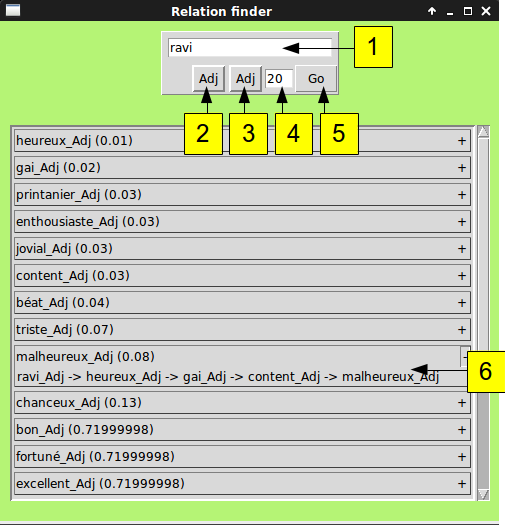
\includegraphics[width=13cm]{relationfinderinterface.png}
\end{center}

\begin{enumerate}
    \item{L'utilisateur peut écrire un mot à rechercher ici}
    \item{Le choix de catégorie syntaxique du mot source parmi une liste 
    d'options. L'option ``*" par défaut signifie que le mot recherché peut être 
    de n'importe quelle catégorie}
    \item{Le choix de catégorie des mots cibles. La liste d'options est la même 
    que pour la catégorie source et peut ne pas correspondre à la catégorie 
    source.}
    \item{Le nombre de voisins à renvoyer. Dans le cas où un mot est relié à 
    moins de voisins que demandé, le maximum de voisins sera renvoyé.}
    \item{Pour lancer une recherche sur le réseau}
    \item{Les voisins sont affichés avec leur distance entre parenthèses. Le 
    chemin est affiché en cliquant sur le signe \lq{+}\rq{}}   

\end{enumerate}

\subsubsection{Optimisation}

L'objectif principal est de maximiser le nombre de mots trouvés qui 
correspondent à la relation de synonymie. Le fait que les paramètres différents 
pour la création et le parcours de la matrice soient des valeurs numériques 
permet d'envisager une optimisation automatique de 
ces valeurs.

Il s'agit, à partir d'un corpus d'entraînement et un vecteur de paramètres de 
regénérer la matrice et évaluer les résultats contre les ressources [REF]XXX 
pour trouver les valeurs qui donnent le meilleur score.

La bibliothèque Scipy fournit une méthode \lq{minimize}\rq{} qui sert à 
minimiser la valeur retourner d'une fonction à partir d'un vecteur de 
paramètres.

\subsubsection{WOLF}

Le corpus WOLF a été réalisé à partir du Princeton WordNet et diverses autres 
ressources multilingues. Il a été évalué par rapport au WordNet français.

Dans le corpus WOLF nous n'avons récupéré que les données ayant été validées 
manuellement. Pour être sûrs de ne pas avoir de bruit dû à quelques ambiguïtés.

Notre extrait de wolf contient 120 mots ainsi que leurs synonymes dans le 
corpus. Chaque mot possède entre 1 et 8 synonymes.

\subsubsection{Crisco}

Le dictionnaire de synonymes Crisco a été réalisé par le laboratoire éponyme 
spécialisé dans l’analyse de l’articulation entre syntaxe et sémantique.

Le corpus Crisco est un petit corpus que nous avons réalisé nous-même pour voir 
si la source du corpus pouvait modifier grandement ou non le score obtenu lors 
de l'évaluation. Nous avons créé ce corpus en entrant les différents mots dans 
la base de données Crisco disponible en ligne.

Notre corpus est composé de 78 mots ayant chacun entre 1 et 10 synonymes.


\subsubsection{Métrique}

Le vecteur de paramètres comprend les valeurs associées aux types de relations 
(ex: pos2entry, sense2deftext, ...) et d'autres paramètres. La récupération de 
ce vecteur est incorporée dans le programme 
pour la création de la matrice, qui contient aussi des méthodes pour changer 
les valeurs de ces paramètres et pour les réécrire dans les fichiers de 
configuration.

L'évaluation selon le corpus se fait en utilisant une métrique que nous 
avons nous-même définie pour juger de la qualité des résultats renvoyés par la 
recherche. Etant donné que les premiers mots dans la liste sont censés être les 
plus proches du mot cible, il est important d'incorporer une notion de 
l'emplacement d'un synonyme trouvé dans la liste de résultats.


\subsection{Evaluation}

L'évaluation de RelationFinder s'est faite en deux temps. D'abord grâce à des 
données récupérées dans le corpus WOLF puis grâce à des données récuppérées sur 
le site de Crisco.

Pour faire cette évaluation nous regardons le mot à traiter puis nous cherchons 
ses k plus proches voisins (dans notre évaluation k = 19). Si l'un des 
synonymes du corpus est dans les k plus proches voisins. On donne un score à ce 
synonyme.

Le score est calculé par rapport à la place du synonymes dans la liste des 
voisins. Si le synonyme est 3ème sur les 19 voisins, il aura un score de 19 - 3 
=\textgreater 16. Si il est 17ème il aura un score de 19 - 17 =\textgreater 2.

Dans le même temps nous calculons le score maximum qu'il est possible 
d'obtenir. C'est-à-dire k - len(syns). Si dans le corpus nous avons 5 synonymes 
alors le score maximum sera 19 + 18 + 17 + 16 + 15 =\textgreater 85.

Pour calculer l'exactitude de notre RelationFinder nous finissons donc par 
diviser le score de tous nos synonymes trouvés par le score maximum total.

Il faut donc bien noter que k ne doit pas être inférieur au nombre maximal de 
Synonymes sinon les résultats peuvent tomber en négatif \dots

\subsubsection{Résultats obtenus}

Lors de l'évalutation nous avons choisi k en fonction du résultat obtenu sur 
le Littré avec le corpus WOLF.

Les scores peuvent aller de 0 à 1. 0 signifierait qu'aucun synonyme dans la 
liste gold n'a été trouvé par RelationFinder tandis que 1 signifierait que 
RelationFinder à trouvé tous les synonymes et qu'ils étaient les premiers mots 
en relation avec le mot cible.

\begin{enumerate}
 \item {Littré :
	\begin{enumerate}
	 \item WOLF :  0,306
	 \item Crisco : 0,145
	\end{enumerate}
	}
 \item {Wiktionnaire :
	\item WOLF : 0,310
	\item Crisco : 0,121
	}
\end{enumerate}

Ces scores sont relativement bas mais cela peut s'expliquer par le fait que le 
RelationFinder ne trouve pas que des synonymes mais aussi des antonymes, 
hyperonymes, etc. Pour améliorer le résultat il suffirait donc d'ajouter 
tout mot sémantiquement lié au mot que l'on évalue \dots 



\section{Désambiguation}
\subsection{Programme}

La deuxièmme tâche que nous nous sommes donnée est la désambiguisation des mots
en contexte. Cela consiste à calculer la distance entre, d'une part, une
phrase entrée par l'utilisateur et, d'autre part, chaque définition du mot à
disambiguïser. Le programme va alors calculer un vector pour chaque couple
(phrase / définition) et la définition renvoyée sera celle ayant le vecteur le
plus important. 

\subsection{Evaluation}


\section{Le Bras Droit du Cruciverbiste (i.e. La Résolution de Mots Croisés)}

La troisième tâche est la résolution d'indices de mots croisés. Le concept est simple et ressemble aux tâches précédentes dans son exploitation du réseau sémantique. Tandis que le chercheur de synonymes calcule la distance entre des mots individuels et le désambiguïseur trouve la distance entre deux séquences de mots, le resolveur de mots-croisés cherche la distance entre une séquence de mots (l'indice) et un mot (le mot cible). Comme précédemment, le noyau du programme est donc une recherche dans la matrice de relations pour trouver un certain nombre de mots candidats. Par contre, des étapes supplémentaires sont nécessaires pour faire en sorte que les mots cibles adhèrent à certaines contraintes imposées par le jeu.

Le principe des mots croisés est de remplir une grille de lettres en fonction d'indices, et en fonction des deux contraintes qui sont la longueur des mots cibles et les caractères qui ont déjà été devinés dans la grille. Notre application est un outil support qui permet de fournir des mots candidats au cruciverbiste\footnote{Un amateur de mots croisés}. A part ces deux contraintes, il est important que les mots candidats correspondent à la catégorie syntaxique indiquée par l'indice. Notons que pour l'instant l'application ne détecte que les mots des catégories \lq{nom}\rq, \lq{adj}\rq, \lq{adv}\rq{} et \lq{verbe}\rq, puisque les autres catégories ne sont pas présentes dans le réseau. Par exemple, pour l'indice \lq{escroqués}\rq, les mots candidats doivent être des participes passés qui sont conjugués au masculin pluriel, et pour l'indice \lq{a l'air chouette}\rq, les mots candidats doivent être des verbes conjugués à la troisème personne singulier du présent indicatif\footnote{Les bonnes réponses sont \lq{eus}\rq{}  et \lq{ulule}\rq{} respectivement}.

Le processus suivi est donc séquentiel et peut être représenté par le schéma suivant:   

\begin{figure}[!ht]
\centering
\def\svgwidth{\columnwidth}
\input{crossword_schema.pdf_tex}
\caption{Le schéma du traitement pour la résolution des indices de mots croisés}
\label{fig:schema_crosswords}
\end{figure}

\subsection{Les étapes de traitement}

\subsubsection{Etape 1 : Identification de la catégorie syntaxique du mot cible}%\label{sec:crossetape1}
Les indices sont de petites séquences de mots qui sont très rarement des phrases complètes et bien formées. Ils correspondent souvent à un syntagme particulier et contiennent parfois des ambiguïtés de catégorie syntaxique dont il faut tenir compte. Il est aussi possible à cette étape d'identifier quelques marques de flexion qui peuvent indiquer la forme du mot cible. Le réseau sémantique ne contient a priori que des lemmes et donc il est important de garder ces indices flexionnels pour re-fléchir les mots candidats à l'étape 3. %(Voir section~\ref{sec:crossetape3).  

Un étiqueteur syntaxique automatique tel que MElt[\hyperref[bib:melt]{~\ref*{bib:melt}}] est peu adapté pour cette identification puisqu'il se base sur les probabilités pour renvoyer la séquence de tags la plus probable pour l'indice. Ceci signifie que le tag prédit peut ne pas correspondre à un des tags possibles pour un mot donné ou les ambiguïtés peuvent ne pas être trouvées. De plus, de tels étiqueteurs sont dépendants de leurs données d'entraînement, et les indices des mots croisés sont d'une forme très différente des données du French TreeBank sur lequel MElt a été entrainé. Nous choisissons donc de faire une analyse point à point des mots de l'indice afin de renvoyer toutes les possibilités catégorielles pour chaque mot. Le Lefff (Lexique des Formes Fléchies du Français)[\hyperref[bib:lefff]{~\ref*{bib:lefff}}] est utilisé pour retrouver toutes les catégories syntaxiques et marques flexionnelles de chaque mot. Cette méthode renvoie évidemment plus de séquences possibles de catégories syntaxiques que souhaitées et crée donc de l'ambiguïté artificielle. Cependant, c'est un moyen d'augmenter le rappel des résultats, même si la précision en souffre. Il est important pour nous de renvoyer le plus de mots candidats possibles et une erreur d'étiquetage syntaxique à cette étape peut significativement nuire les chances de trouver les bons candidats par la suite.

La catégorie syntaxique du mot cible peut être identifiée à partir de la séquence d'ensembles de catégories grâce à la régularité des formes des indices. Si un indice contient un seul mot, les catégories cibles sont celles du mot de l'indice. Sinon, la catégorie dépend en grande partie des premiers mots de l'indice. Par exemple, si un indice commence par un nom, ou une séquence \lq{det nom}\rq{} ou une séquence \lq{det adj nom}\rq{}, la catégorie cible, étant donné qu'il n'y a pas d'ambiguïté catégorielle, serait un nom. Dans certains cas, il est aussi possible d'identifier quel mot de l'indice indique la flexion du mot cible. Cette identification se fait à l'aide d'une mini-grammaire de seulement 18 règles, qui sont reproduites ci-dessous :

\begin{framed}
det nc -\textgreater 2, nc\newline
det adj nc -\textgreater 3, nc\newline
adj nc -\textgreater 2, nc\newline
nc -\textgreater 1, nc\newline
adj prep -\textgreater 1, adj\newline
adv v -\textgreater 2, v\newline
advm v -\textgreater 2, v\newline
advneg v -\textgreater 2, v\newline
advneg advneg v -\textgreater 3, v\newline
v -\textgreater 1, v\newline
clr v -\textgreater 2, v\newline
prel v -\textgreater 2, adj \newline
cln v -\textgreater 2, n\newline
prep nc -\textgreater ?, adv\newline
ce v det nc -\textgreater 4, nc\newline
adj coo adj -\textgreater 1, adj\newline
nc coo nc -\textgreater 1, adj\newline
pri v -\textgreater 2, adj
\end{framed}

Chaque ligne représente une règle différente. A gauche de la flèche est la séquence de mots qui indique, au début d'un indice, une certaine catégorie syntaxique pour le mot cible. A droite de la flèche est l'indice (à partir de 1) du mot de la partie gauche dont les informations grammaticales seront utilisées pour fléchir les mots cibles (qui seront des lemmes), suivi de la catégorie syntaxique du mot cible. Dans le cas où aucun mot de l'indice en particulier donne des indices flexionnels, \lq{?}\rq{} indique que les indices flexionnels sont inconnus. Par exemple, un indice tel que \lq{avec soin}\rq{} correspond à la règle \lq{prep nc -\textgreater ?, adj}\rq{}, où la catégorie cible serait \lq{adv}\rq{}, mais où aucun mot entre la préposition et le nom fournit d'indice flexionnels.

Le jeu d'étiquettes utilisées est celle du Lefff\footnote{Ce jeu a été réduit pour ne contenir que les noms, adjectifs, adverbes et verbes et les catégories nécessaire pour la mini-grammaire}, qui est utilisé pour retrouver les formes fléchies. Un même indice peut correspondre à plusieurs règles différentes si un mot donné est ambigu pour la catégorie syntaxique.

Les catégories syntaxiques sont retenues pour le parcours du réseau et les informations grammaticales pour retrouver les formes fléchies correspondant aux lemmes trouvés dans le réseau.

Remarque : Une particularité des indices est que parfois elles peuvent contenir plusieurs parties, séparées d'une virgule et qui représentent plusieurs sous-indices à l'intérieur de l'indice. Par exemple, un indice peut avoir la forme \lq{habillée, fringuée}\rq{} et dans ce cas, il est souhaitable de séparer cet indice en \lq{habillée}\rq{} et \lq{fringuée}\rq{} afin d'avoir la meilleure chance de trouver la catégorie voulue. Idéalement, ces deux parties devraient aussi correspondre en termes de catégorie syntaxique, ce qui signifie qu'il faudrait en théorie ne garder que les catégories cibles qui correspondent aux deux parties de l'indice. Par contre, nous optons pour le choix de garder toutes les catégories potentielles à partir des deux parties de l'indice pour nous assurer de la couverture maximale. 

\subsubsection{Etape 2 : Recherche dans le graphe}%\label{sec:crossetape2}

Une fois que la catégorie syntaxique de la solution est ciblée (ou au moins 
réduite à une liste de catégories possibles), et les mots de l'indice sont 
lemmatisés, il est possible d'utiliser le réseau sémantique pour trouver les 
mots les plus proches à l'indice. Ici nous testons la première stratégie de 
recherche dans le graphe: l'algorithme de parcours en largeur pour renvoyer les 
k plus proches voisins de chaque lemme. Une extension serait d'implémenter aussi 
la recherche de la matrice complète. Le choix des plus proches candidats va 
dépendre de l'algorithme utilisé.

Un indice peut contenir plusieurs lemmes et avec le réseau sémantique, il est facile de renvoyer les voisins (avec leurs distances) d'un mot individuel. Pour le parcours en largeur il s'agit de parcourir le graphe jusquà'ce que les k plus proches voisins sont trouvés. Dans la matrice complète il est possible d'atteindre la liste complète des sommets du réseau avec leurs distances du mot recherché. 

Les voisins d'un lemme donné peuvent être vu comme un vecteur où les paramètres sont les voisins et les valeurs sont leurs distances du lemme. Par exemple un indice \lq{lemme1 lemme2 lemme3}\rq{} aurait trois vecteurs différents pour représenter chacun des lemmes, chacun avec un certain nombre de paramètres spécifiés (en fonction de l'algorithme de recherche utilisé), qui ne seront pas forcément les mêmes pour chaque vecteur (si seulement les k plus proches sont trouvés):

\begin{framed}
vec\_lemme1 : \textless{a: 1, b: 2, c: 3}\textgreater \newline
vec\_lemme2 : \textless{a: 1, b: 5, d: 4}\textgreater \newline
vec\_lemme3 : \textless{a: 4, c: 1, e: 1}\textgreater 
\end{framed}

Le vecteur global doit être représentatif des trois lemmes et des paramètres que contiennent leurs vecteurs. Si la matrice complète est utilisée, les vecteurs des lemmes contiendraient les mêmes voisins est un moyennage des distances est possible pour chaque voisin. Par contre, un moyennage simple des valeurs n'est pas possible pour le parcours en largeur, puisque les voisins non-représentés auraient une valeur infinie pour la distance, ce qui fausserait les distances moyennées. Le choix dans ce cas-là est donc d'ajouter les vecteurs pour en faire un vecteur global, et dans le cas où un paramètre apparaît dans plusieurs vecteurs, comme ci-dessus avec \lq{a}\rq{}, \lq{b}\rq{} et \lq{c}\rq{}, la distance minimale est choisie. Les trois vecteurs ci-dessus aurait alors comme vecteur global:

\begin{framed}
vec\_indice : \textless{a: 1, b: 2, c: 1, d: 4, e: 1}\textgreater 
\end{framed}

Remarques sur les formes recherchées : les lemmes des mots de l'indice sont recherchés dans le réseau, suffixés de leurs catégories syntaxiques possibles, ce qui signfie qu'un mot qui est syntaxiquement ambigu sera recherché plusieurs fois. Si le lemme ne se trouve pas dans le Lefff, au lieu d'abandonner la recherche de ce mot, nous utilisons le mot-forme par défaut, en espérant que ce mot appartient au réseau (particulièrement important pour les noms propres par exemple).\footnote{Même si le réseau ne devraient pas contenir de formes fléchies, il est possible qu'il en contient à cause des erreurs de tagging, et donc nous exploitons cette faiblesse ici pour augmenter la chance de retrouver le plus de mots de l'indice possibles.}. Les catégories syntaxiques cibles sont celles obtenues à partir de la mini-grammaire est en cas de non-identification de catégorie, des candidats de toute catégorie seront recherchés.

\subsubsection{Etape 3 : Conjugaison des lemmes obtenus}%\label{sec:crossetape3}

Les résultats de la recherche du graphe sont (pour la plupart) des lemmes, qui
sont à modifier pour correspondre à la forme du mot recherché. En utilisant 
l'ensemble de catégories et d'informations grammaticales obtenues lors de 
l'étape 1, cette étape cherche les formes fléchies correspondant à chaque 
lemme et vérifie lesquelles correspondent aux informations grammaticales 
recherchées pour les mots candidats.

La ressource utilisée est encore une fois le Lefff, avec pour chaque lemme qui y apparaît, ces catégories syntaxiques possibles et les formes fléchies associées. En connaissant les catégories syntaxiques possibles pour le mot cible (obtenues à l'étape 1), les formes fléchies du lemme sont triées en fonction de leur correspondance aux informations grammaticales aussi obtenues à l'étape 1. Si un trait grammatical (ex: 'nombre') est exprimé pour les flexions voulues, la forme fléchie sera retenue seulement si elle a la même valeur de trait (pourvu que ce trait soit exprimé).

Par exemple, si l'indice est \lq{mangée}\rq{}, les informations grammaticales retenues sont que la catégorie est un participe passé et que le mot recherché doit être féminin singulier. Les voisins du lemme \lq{manger}\rq{} seront recherchés dans le réseau et renvoyés:

\begin{framed}
consommer, alimenter, boire etc.
\end{framed}

Il existe un grand nombre de formes fléchies de ces verbes, mais dont un petit nombre correspondent aux contraintes grammaticales \lq{féminin singulier}\rq{}. Les formes suivantes seront alors rejetées:

\begin{framed}
consommâtes, consommèrent, consommé, consomme, ..., alimentez, alimentées, etc.
\end{framed}

et les formes suivantes retenues:

\begin{framed}
consommée, alimentée, bue
\end{framed}

\subsubsection{Etape 4 : Filtrage selon les contraintes}%\label{sec:crossetape4}

La dernière étape filtre les candidats fléchis afin de ne renvoyer que les candidats qui se conforment aux contraintes de longueur de mot et de caractères déjà devinés. Il n'est pas possible de faire cette étape avant la conjugaison, puisque la conjugaison des lemmes peut avoir pour effet un changement dans la longueur du mot et des caractères qui y apparaîssent.

Souvent dans les outils d'aide de résolution de mots fléchés, cette étape est la seule incluse dans le programme, et donc un grand nombre de mots correspondent aux contraintes de longueur et de caractères. Dans notre programme, cette étape sert à enlever la grande quantité de bruit dans les résultats produits directement à partir du réseau, et permet de raffiner en grande partie les résultats. L'avantage d'utiliser le réseau est qu'il y a plus de chance d'avoir des résultats qui correspondent à l'indice donné et non pas des mots candidats indépendant de l'indice, ce qui permet un traitement plus sophistiqué à cette étape.

\subsection{L'interface graphique}

L'interface graphique, implementée en python en utilisant les bibliothèques 
Tkinter et PMW sert à visualiser les résultats renvoyés aux différentes 
étapes du processus. Elle est mi-chemin entre un outil pour un joueur de mots 
croisés, qui ne s'intéresse qu'aux mots qui se conforment aux contraintes 
données et un outil plus pédagogue pour montrer les étapes du traitement.

\begin{center}
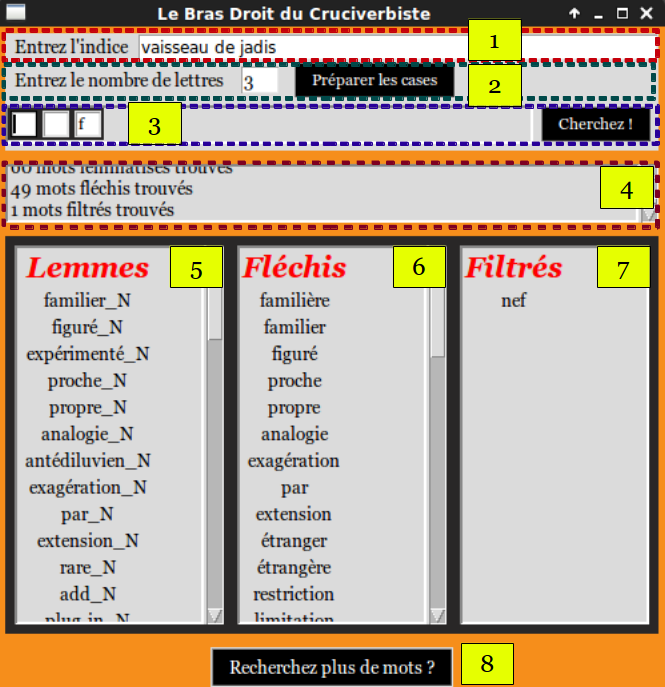
\includegraphics{CrossWordInterface.png}
\end{center}

\begin{enumerate}
    \item{L'indice qui sert à deviner le mot recherché}
    \item{Le nombre de lettres du mot recherché. En cliquant sur \lq{Préparer les cases}\rq, cette contrainte sera enregistrée et les cases générées en 3.}
    \item{Les cases pour entrer les caractères déjà devinés. Cette contrainte sera prise en compte dans le filtrage des mots candidats}
    \item{Le log qui permet de tracer le suivi du programme. Ici seront affichés des avertissements dans le cas où un mot n'est pas reconnu, la/les catégorie(s) syntaxique(s) du mot recherché et le nombre de résultats renvoyés à chaque tour.}
    \item{Les plus proches voisins de l'indice. Au départ les vingt mots les plus proches seront retournés.}
    \item{Les formes fléchies des lemmes renvoyés en 5., qui devraient correspondre aux contraintes flexionnelles imposées par les mots de l'indice, si elles sont reconnues}
    \item{Les candidats filtrés selon les contraintes de longueur de mot et de caractères déjà devinés.}
    \item{Si l'utilisateur veut continuer en regardant les vingt prochains plus proches mots, il peut cliquer sur ce bouton pour renvoyer plus de résultats. Ceci peut être utile dans le cas où peu de résultats fléchis ou filtrés sont renvoyés.}
    
\end{enumerate}


\subsection{Evaluation}
Le système est difficilement évaluable contre d'autre systèmes de la même nature, parce qu'il n'existe pas de système d'évaluation standard et de scores comparatifs. Il existe beaucoup de systèmes qui ne se basent pas sur la similarité sémantique, mais qui renvoient plutôt tous les mots possibles qui correspndent aux contraintes de longueur et de caractères déjà devinés, et ces systèmes ne fournissent pas un bon moyen de comparer l'approche par réseau sémantique, qui fournit moins de formes globalement.

Notre évaluation est donc une évaluation simple de la capacité du réseau à 
trouver la solution d'un indice, et qui compare le taux de réussite pour 
différents niveaux de difficulté et pour différentes catégories syntaxiques. 
L'évaluation se fait sur un petit corpus d'indices pris d'un site internet de 
mots fléchés (\hyperref[bib:mfg]{[~\ref*{bib:mfg}]})qui classe les grilles par 
niveaux. Le corpus se trouve dans l'annexe. Il est vrai 
que l'emplacement des mots dans la grille les uns par rapport aux autres 
contribue au niveau global de la grille, mais nous estimons que le niveau est 
aussi reflété dans la difficulté des indices individuels. Le corpus contient 
deux niveaux différents (1 et 2) et pour chaque niveau vingt noms communs, vingt 
noms propres, vingt adjectifs et vingt verbes. Les indices étaient pris aussi 
objectivement que possible, avec soin de ne pas répéter le même mot cible entre 
deux indices, ou de prendre exclusivement des indices qui contiennent une seule 
tournure. Autant de solutions de chaque catégorie ont été sélectionnées afin de 
comparer le taux de réussite pour chaque catégorie, mais le constat a été que le 
niveau contient plus de noms communs et moins de nom propres, ce qui influence 
aussi la difficulté des indices.

A part le but principal de trier les mots candidats par rapport à la similarité sémantique, les choix de traitement sont clairement orientés vers une optimisation du rappel (par exemple, le choix de faire une analyse morphologique point à point). Le système d'évaluation se juge donc sur le rappel des résultats. Pour chaque indice, nous cherchons d'abord si la solution apparaît dans le réseau et si oui, après combien de voisins les plus proches le mot est trouvé. Pour éviter de parcourir tout le réseau en cas de non-découverte, nous limitons le maximum de voisins renvoyés à 200. Au délà de 200, le mot est considéré non-trouvé. Une analyse détaillée se trouve ci-dessous :

\begin{table}[ht]
\centering
\begin{tabular}{|p{0.8cm} |p{0.8cm} |p{0.8cm}| p{0.8cm} |p{0.8cm}|p{0.8cm}|p{0.8cm}|p{0.8cm}|p{2.8cm}}
%\multicolumn{1}{c}{Level} & \multicolumn{4}{c}{Solution trouvée} \\[0.5ex]
\hline
 &  &  & \multicolumn{5}{c}{Solution trouvée après ...} & \\[0.5ex]
\hline
Level & POS & \# & 20 & 40 & 160 & 180 & 200 & Non-trouvée\\[0.5ex]
\hline
\hline
1 & Adj & 20 & 3 & 0 & 1 & 0 & 1 & 15 \\[0.5ex]
\hline
1 & NC & 20 & 1 & 0 & 0 & 0 & 0 & 19 \\[0.5ex]
\hline
1 & NP & 20 & 1 & 0 & 0 & 0 & 0 & 19 \\[0.5ex]
\hline
1 & V & 20 & 1 & 0 & 0 & 0 & 0 & 19 \\[0.5ex]
\hline
2 & Adj & 20 & 1 & 0 & 0 & 0 & 0 & 19 \\[0.5ex]
\hline
2 & NC & 20 & 1 & 0 & 0 & 0 & 0 & 19 \\[0.5ex]
\hline
2 & NP & 20 & 0 & 0 & 0 & 0 & 0 & 20 \\[0.5ex]
\hline
2 & V & 20 & 0 & 0 & 0 & 0 & 0 & 20\\[0.5ex]
\hline
\end{tabular}
\caption{Résultats de la recherche pour chaque niveau et chaque catégorie syntaxique à partir du Wiktionnaire}
\label{table:resultscrosswords}
\end{table}

\begin{table}[ht]
\centering
\begin{tabular}{|p{1.8cm}|p{1.8cm}|p{1.8cm}|p{1.8cm}|p{1.8cm}|p{1.8cm}|p{1.8cm}|}
%\multicolumn{1}{c}{Level} & \multicolumn{4}{c}{Solution trouvée} \\[0.5ex]
\hline
Level x & POS & Nombre & POS identifié & Solution dans le réseau & Solution dans le Lefff & Pas de voisins\\[0.5ex]
\hline\hline
1 & Adj & 20 & 14 & 19 & 19 & 1 \\[0.5ex]
\hline
1 & NC & 20 & 17 & 16 & 16 & 1 \\[0.5ex] 
\hline
1 & NP & 20 & 19 & 4 & 4 & 0 \\[0.5ex]
\hline
1 & Verbe & 20 & 19 & 18 & 18 & 0 \\[0.5ex]
\hline
2 & Adj & 20 & 12 & 18 & 18 & 0 \\[0.5ex]
\hline
2 & NC & 20 & 18 & 18 & 18 & 0 \\[0.5ex] 
\hline
2 & NP & 20 & 17 & 1 & 1 & 0 \\[0.5ex]
\hline
2 & Verbe & 20 & 19 & 19 & 19 & 0 \\[0.5ex]
\hline
\end{tabular}
\caption{Analyse du processus à partir des résultats du Wiktionnaire}
\label{table:anaprocesscrosswords}
\end{table}

Malgré le fait que le nombre de solutions trouvées soit très bas (10 sur un total de 160), ces résultats montrent qu'un réseau sémantique, même très peu sophistiqué et en utilisant un algorithme de recherche très simple, peut, dans certains cas, servir d'outil pour retrouver un mot à partir d'un ensemble de mots indicateurs. A partir de ces bases, il serait possible dans de futurs travaux d'améliorer le réseau afin de maximiser ces scores. La catégorie syntaxique pour laquelle la solution a été trouvée le plus souvent est l'adjectif (6 sur les 10 solutions trouvées). Le niveau 1 a fourni plus de candidats corrects pour cette catégorie (3) que le niveau 2 (1), ce qui peut refléter la difficulté de niveau dans les indices et une similarité sémantique moins directe entre l'indice et la solution pour le niveau 2. Les catégories pour qui le moins de solutions ont été trouvées sont les noms propres et les verbes. Ce n'est pas étonnant que les noms propres reçoivent un faible score, puisque ces formes sont moins représentées dans les dictionnaires en général que les nom communs et risquent d'avoir moins de liens avec d'autres termes plus fréquents. Pour les verbes, il est possible qu'il existe trop de bruit dans le réseau dû au fait que les verbes sont fréquemment utilisés dans les définitions pour des raisons non-basées sur la similarité sémantique telle que la synonymie. Les adjectifs par contre sont souvent utilisés pour les descriptions au lieu de la structuration syntaxique des définitions et donc les liens établis avec les adjectifs peuvent avoir tendance à être plus pertinente pour juger des relations entre les mots.

Le comptage des solutions trouvées se fait par étapes de 20. L'étape 20 indique le nombre de solutions trouvées après que les premiers 20 plus proches voisins de chaque mot de l'indice ont été utilisés. L'étape 40 indique le nombre de solutions trouvées après que les premiers 40 plus proches voisins de chaque mot ont été utilisés. Ce qui est intéressant est que la plupart des solutions (8/10) ont été trouvé en utilisant seulement les vingt premiers voisins de chaque mot de l'indice. Après cette première séries de voisins retournés, très peu de solutions ont été trouvées (seulement un adjectif de niveau 1 après 160 voisins et un adjectif de niveau 1 après 200 voisins). Ces résultats indiquent que les solutions trouvées n'ont pas été trouvées par hasard, sinon on s'attendrait à voir autant de solutions dans les étapes de recherche suivantes. Le nombre de solutions trouvées dans cette première colonne de 20 vingt voisins est relativement peu par rapport au nombre d'indices recherchés, mais ces résultats sont encourageants puisqu'ils montrent que la similarité sémantique a servi dans ces cas pour trouver la bonne solution.

L'analyse du processus montrée dans la table \hyperref[table:anaprocesscrosswords]{Figure~\ref*{table:anaprocesscrosswords}} montre à quel point l'application est adaptée à la tâche. Un premier test de la présence des lemmes des solutions dans le réseau et des formes fléchies des solutions dans le Lefff permet de voir que la plupart des solutions apparaissent dans les deux ressources. Ceci est encourageant; si le lemma de la solution n'est pas trouvable dans le réseau, il n'y aucune chance de trouver le bon résultat, et si le lemme diffère de la forme fléchie et cette forme n'apparaît pas dans le Lefff, la solution n'est pas non plus trouvable. Ici les résultats sont un peu trivial par rapport au nombre de solutions trouvées dans le réseau et dans le Lefff, parce que les chiffres sont identiques pour chaque catégorie syntaxique. La raison pour ces chiffres est que si la forme n'apparaît pas dans le Lefff, on ne peut pas retrouver automatiquement sa forme et donc il y a au moins le même nombre de mots non trouvés dans le Lefff que dans le réseau. Il faudrait un deuxième outil pour détailler plus ce point. Pour la plupart des catégories au moins 18/20 solutions étaient dans le réseau et le Lefff et pourraient a priori être sélectionnées comme mot candidat. Ce chiffre est un peu moins élevé pour les noms communs de niveau 1, ce qui montre une plus petite couverture pour ces indices, qui pourrait être dû au choix des indices spécifiques. Par contre la couverture pour les noms propres est très faible, avec seulement un nom propre sur 20 étant trouvé pour le niveau 2.

Ce qui est intéressant est que la couverture pour les mots des indices est relativement grande. La dernière colonne \lq{Pas de voisins}\rq indique pour combien d'indices aucun voisin a été trouvé, souvent dans le cas où aucun mot de l'indice apparaît dans le réseau. Ce cas s'est produit seulement 3 fois sur les 160 indices testés. De plus, une grande majorité des catégories syntaxiques cibles ont été correctement identifiées, avec 19/20 pour les noms propres de niveau 1, les verbes de niveau 1 et les verbes de niveau 2. Ceci indique que, en général, les mots des indices se sont apparus dans le Lefff et que la catégorie syntaxique des mots porteurs étaient identifiées pour attribuer une catégorie cible pour l'indice entière. Notons qu'une distinction n'a pas été faite entre les noms propres et les noms communs dans la recherche dans le réseau, dans lequel les deux sont de catégorie \lq{nom}\rq. Pour les noms propres, cette grande différence entre la couverture de l'indice et des solutions est probablement dûe au fait que les indices contiennent souvent une description du nom propre en utilisant des noms communs et que les solutions soient des noms propres pour lesquels la couverture est petite. La catégorie syntaxique la moins bien identifiée est l'adjectif, à 14/20 pour le niveau 1 et 12/20 pour le niveau 2. Nous constatons que ces catégories sont difficiles à identifier à cause du grand débat du statut des adjectifs et des participes passés. Souvent, un mot qui pourrait être considéré comme à la fois un adjectif et un participe passé, tel que \lq{fatigué}\rq{} est plus souvent marqué comme un participe passé qu'un adjectif, ce qui est parfois le cas dans le Lefff, ce qui peut mener à une mauvaise identification de la catégorie cible. 
   
\subsection{Améliorations possibles}
Nous avons vu que le problème principal de l'application n'est pas que les solutions n'apparaissent dans le réseau sémantique, et elles sont a priori trouvables. Le problème est qu'il n'existe pas suffisamment de liens pertinents entre les mots de l'indice et les solutions, surtout pour les niveaux plus difficiles, qui contiennent des termes moins directement liés aux solutions.

L'identification de la catégorie syntaxique a un assez bon rappel, mais est très bruitée à cause d'une grande quantité d'ambiguïté morphologique produite par l'analyse morphologique point à point. Une meilleure solution serait d'entraîner un étiqueteur syntaxique tel que MElt sur les données similaires aux mots d'indices afin de mieux l'adapter à nos données et d'avoir une identification plus précise de la catégorie. L'ambiguïté artificielle que notre application a produite a pour effet un bruitage des voisins renvoyé, puisque toutes les catégories différentes peuvent être renvoyées. De plus, chaque fois qu'il existe une ambiguïté morphologique pour un mot de l'indice, autant de vecteurs de 20 voisins sont produits pour ce mot qu'il a de catégories syntaxiques possible, ce qui peut aussi ajouter du bruit aux résultats.

Une amélioration importante serait d'augmenter la couverture des noms propres, qui sont particulièrement utilisés dans les niveaux plus élevés de mots-croisés. Dans ce cas, il faudrait aussi faire la distinction entre nom commun et nom propre afin de ne pas renvoyer des noms propres au lieu de noms communs.

Il serait possible de chercher plus de voisins dans le réseau pour augmenter la possibilité de trouver la bonne solution, mais ceci n'est pas le principe du réseau. Il existe déjà des outils qui renvoient tous les mots qui peuvent correspondre aux contraintes de longueur et de caractères déjà devinés, et notre méthode cherche à trouver un moyen de renvoyer les solutions plus pertinentes par rapport à la sémantique sans devoir parcourir le réseau entier pour trouver les solutions.









\appendix
\section{Parametres des poids}\label{App:weights}
%\verbatiminput{../Scripts/Matrices/LITTREMatrix_resources/simplifiedweights.config}

\section{Parametres supplémentaires pour la ponderation des aretes}\label{App:otherparams}
Text of Appendix B is Here

\section{Script de normalisation du Littre}\label{App:normlittre}
%\lstinputlisting[language=Python]{../Scripts/XML/LITTRE_normalisation.py}

\section{Script de normalisation du Wiktionnaire}\label{App:normwiki}
Text of Appendix B is Here

\section{DTD des fichiers XML produits}\label{App:dtddico}
Text of Appendix B is Here

\section{Script utilise pour l'etiquetage syntaxique et la lemmatisation}\label{App:tag}
%\lstinputlisting[language=Python]{../Scripts/XML/tagging_modifs3.py}

\section{Script pour la creation de la matrice}\label{App:creatematrix}
Text of Appendix B is Here


\begin{thebibliography}{10}

\bibitem{wordnet}Princeton University "About WordNet." WordNet. Princeton 
University. 2010. http://wordnet.princeton.edu \label{bib:wordnet}

\bibitem{WikiXML}WiktionaryX. 
http://redac.univ-tlse2.fr/lexiques/wiktionaryx.html. 
Franck Sajous. CLLE-ERSS. \label{bib:wikixml}

\bibitem{LittreXML}Littré, Émile. Dictionnaire de la langue française, 
Supplément. Paris, L. Hachette, 1878. Electronic version created by François 
Gannaz. http://www.littre.org \label{bib:littrexml}

\bibitem{MElt}Pascal Denis and Benoît Sagot (2012). Coupling an annotated 
corpus and a lexicon for state-of-the-art POS tagging. In Language Resources 
and Evaluation 46:4, pp. 721-736, DOI 10.1007/s10579-012-9193-0\label{bib:melt} 

\bibitem{lefff}Sagot (2010). The Lefff, a freely available and large-coverage 
morphological and syntactic lexicon for French. In Proceedings of the 7th 
international conference on Language Resources and Evaluation (LREC 2010), 
Istanbul, Turkey\label{bib:lefff} 

\bibitem{olnyetal}Olney J., Revard C. et Ziff P. (1968) Toward the development
 of computational aids for obtaining a formal semantic description of English.
System Development Corporation, Santa Monica\label{bib:olnyetal} 


\bibitem{word2vec}Mikolov T., Chen K., Corrado G. et Dean J. (2013)
Efficient Estimation of Word Representations in Vector Space. In
Proceedings of Workshop at ICLR.\label{bib:word2vec} 

\bibitem{gaumeetal}Gaume B., Hathout N. et Muller P. (2004)
Word Sense Disambiguation using a dictionary for sense similarity measure.
In Proceedings of the 20th international conference on Computational
Linguistics.\label{bib:gaumeetal} 

\bibitem{mulleretal}Muller P., Hathout N. et Gaume B. (2006)
Synonym extraction using a semantic distance on a dictionary.
In Proceding of the First Workshop on Graph Based Methods for
Natural Language Processing.\label{bib:mulleretal} 

\bibitem{traversmilgram}Travers J. et Milgram S. (1969)
An Experimental Study of the Small World Problem.
In Sociometry, Vol 32, No. 4, pp. 425-443\label{bib:traversmilgram} 

\bibitem{wattsstrogatz}Watts D. et Strogatz S. (1998)
Collective dynamics of 'small-world' networks
In Nature Vol 393 (6684), pp. 440-442 \label{bib:wattsstrogatz} 

\bibitem{veronis}Véronis J. (2004)
HyperLex: lexical cartography for information retrieval.
In Computer Speech and Language 18(3) pp 223-252. \label{bib:veronis} 

\bibitem{barabasi}Barabási A. et Albert R. (1999)
Emergence of scaling in random networks.
In Science 286 (5439) pp. 509-512 \label{bib:barabasi}

\bibitem{pagerank}Page L., Brin S., Motwani R. et Winograd T. (1998)
The pagerank citation ranking: Bringing order to the web.
Technical report, Stanford Digital Library Technologies Project.
\label{bib:pagerank}

\bibitem{linkanalysis}Leskovec A., Rajaraman A. et Ullman J. (2010)
Mining of Massive Datasets.
\label{bib:linkanalysis}

\bibitem{lesk}Lesk M. (1986)
Automatic sense disambiguation using machine readable dictionaries:
how to tell a pine cone from an ice cream cone.
In SIGDOC: Proceedings of the 5^{th} annual international conference
on Systems documentations pp 24-26 
\label{bib:lesk}

\end{thebibliography}


\end{document}
